\qns{Transfer Functions from Bode Plots}

\qcontributor{Siddharth Iyer}

\begin{enumerate}

\qitem
  \textbf{Derive a transfer function that would result in the following Bode plot.}
  \begin{figure}[H]\centering
  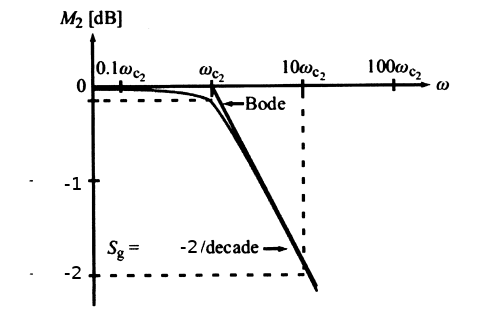
\includegraphics[width=0.4\textwidth]{\bank/transfer/q_bode/bode1_fixed}
  \end{figure}

\sol{

  $$H(\omega) = \frac{1}{\left(1 + \frac{j\omega}{\omega_c}\right)^2}$$
  
}

\qitem
  \textbf{Derive a transfer function that would result in the following Bode plot.}
  \begin{figure}[H]\centering
  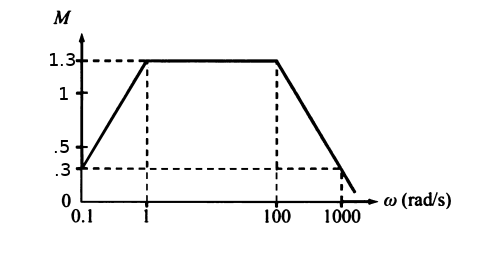
\includegraphics[width=0.4\textwidth]{\bank/transfer/q_bode/bode2_fixed}
  \end{figure}
  \textit{Hint:} $\log_{10} 2 = 0.3$

\sol{

  $$H(\omega) = \frac{j 20 \omega}{\left(1 + j\omega\right)\left(1 + \frac{j\omega}{100}
  \right)}$$
  
}

%\qitem
%  \textbf{OPTIONAL:} Derive the symbolic transfer function for the following circuit.
%
%    \begin{figure}[h!]\centering
  \begin{circuitikz}
    \draw (3.5,2.5) node[op amp, yscale=-1] (opamp1) {}
      (opamp1.+) to[R = $R_2$,-o] (0,3) node[left] {$V_{in}$};
    \draw (1,0) node[ground] {}
      to[R=$R_1$,-] (1, 2)
      |- (opamp1.-)
      to[short,-] (2.3, 1)
      to[R=$R_3$] (4.5, 1)
      -| (opamp1.out) node[above] {$V_x$}
      to[R=$R_5$,*-] (6.5,2.5)
      to[R=$R_6$] (6.5,1) node[ground] {};
    \draw (9.5,2) node[op amp] (opamp2) {}
      (opamp2.+) -| ++(-0.5, -0.5) node[ground] {};
    \draw (6.5,2.5)
      -| (opamp2.-)
      to[short] ++(0,1)
      to[R=$R_7$] ++(2,0)
      -| (opamp2.out)
      to[short,-o] (12,2) node[right] {$V_{out}$};
    \draw (2.3, 1)
      |- (3,0)
      to[R=$R_4$] (6,0)
      -| (11,2);
  \end{circuitikz}
\end{figure}

%
%\sol{
%
%  By the Golden Rules, the inputs to the first op-amp are at $V_{in}$ and the inputs to the second op-amp are at $0$.
%  Using KCL at the negative inputs to the two op-amps,
%  \begin{align*}
%  \frac{V_{in}-V_x}{R_3} + \frac{V_{in}}{R_1} + \frac{V_{in}-V_{out}}{R_4} &= 0\\
%  \frac{-V_{out}}{R_7} + \frac{-V_x}{R_5} &= 0
%  \end{align*}
%  Substituting $V_x = -\frac{R_5 V_{out}}{R_7}$ into the first equation and rearranging,
%  \begin{align*}
%  \frac{V_{in}}{R_3} + \frac{R_5 V_{out}}{R_7 R_3} + \frac{V_{in}}{R_1} + \frac{V_{in}}{R_4} - \frac{V_{out}}{R_4}  &=  0\\
%  \left(\frac{1}{R_3} + \frac{1}{R_1} + \frac{1}{R_4}\right) V_{in}  &= \left(\frac{1}{R_4} - \frac{R_5}{R_7 R_3}\right) V_{out}\\
%  \left(\frac{R_1 R_3 + R_3 R_4 + R_1 R_4}{R_1 R_3 R_4}\right) V_{in}  &= \left(\frac{R_3 R_7 - R_4 R_5}{R_3 R_4 R_7}\right) V_{out}\\
%  \frac{V_{out}}{V_{in}}  &= \frac{\frac{R_1 R_3 + R_3 R_4 + R_1 R_4}{R_1 R_3 R_4}}{\frac{R_3 R_7 - R_4 R_5}{R_3 R_4 R_7}}\\
%  H(\omega) &= \frac{R_3R_4R_7 + R_1R_4R_7 + R_1R_3R_7}{R_1R_3R_7 - R_1R_4R_5}
%  \end{align*}
%  
%}

\end{enumerate}
